\documentclass{article}

\usepackage{graphicx}
\usepackage{lmodern}
\usepackage{enumitem}

\begin{document}
	\begin{titlepage}
		\fontfamily{pbk}\selectfont
		\hbox{			
			\rule{1pt}{\textheight}
			\hspace*{0.05\textwidth}
			\parbox[b]{\textwidth}{
				\Large Project Tender\\[1cm]
					
				\Huge Project: Harvest\\
				\huge Client: Subtrop\\[1.5cm]					
					
				{\huge Team: HTTP\textunderscore418}
				
				\begin{itemize}[label={}, leftmargin=0pt, noitemsep]
					\Large						
					\item Christiaan Saaiman, 12059138
					\item Michael Loosen, 14017254
					\item Elizabeth Bode, 14310156
					\item LC Meyers, 14024633
				\end{itemize}
				\vspace{0.5cm}
					
				{\large Department of Computer Science, University of Pretoria\\[0.2cm]}

				\Large\today\\[0.3cm]				
									
				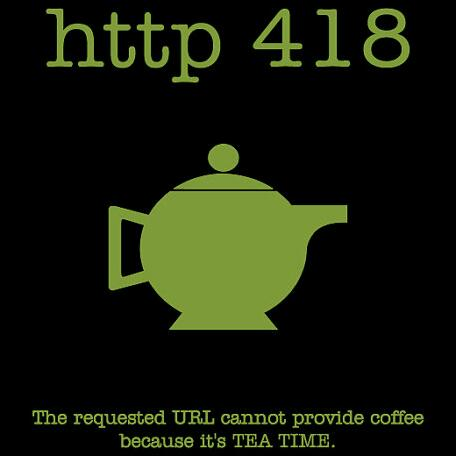
\includegraphics[scale=0.3]{../teamPic.jpg}					
			}								
		}
	\end{titlepage}
	\newpage
	\section{The Team}
	\subsection{LC Meyers}
	\begin{figure}[h]
		\centering
		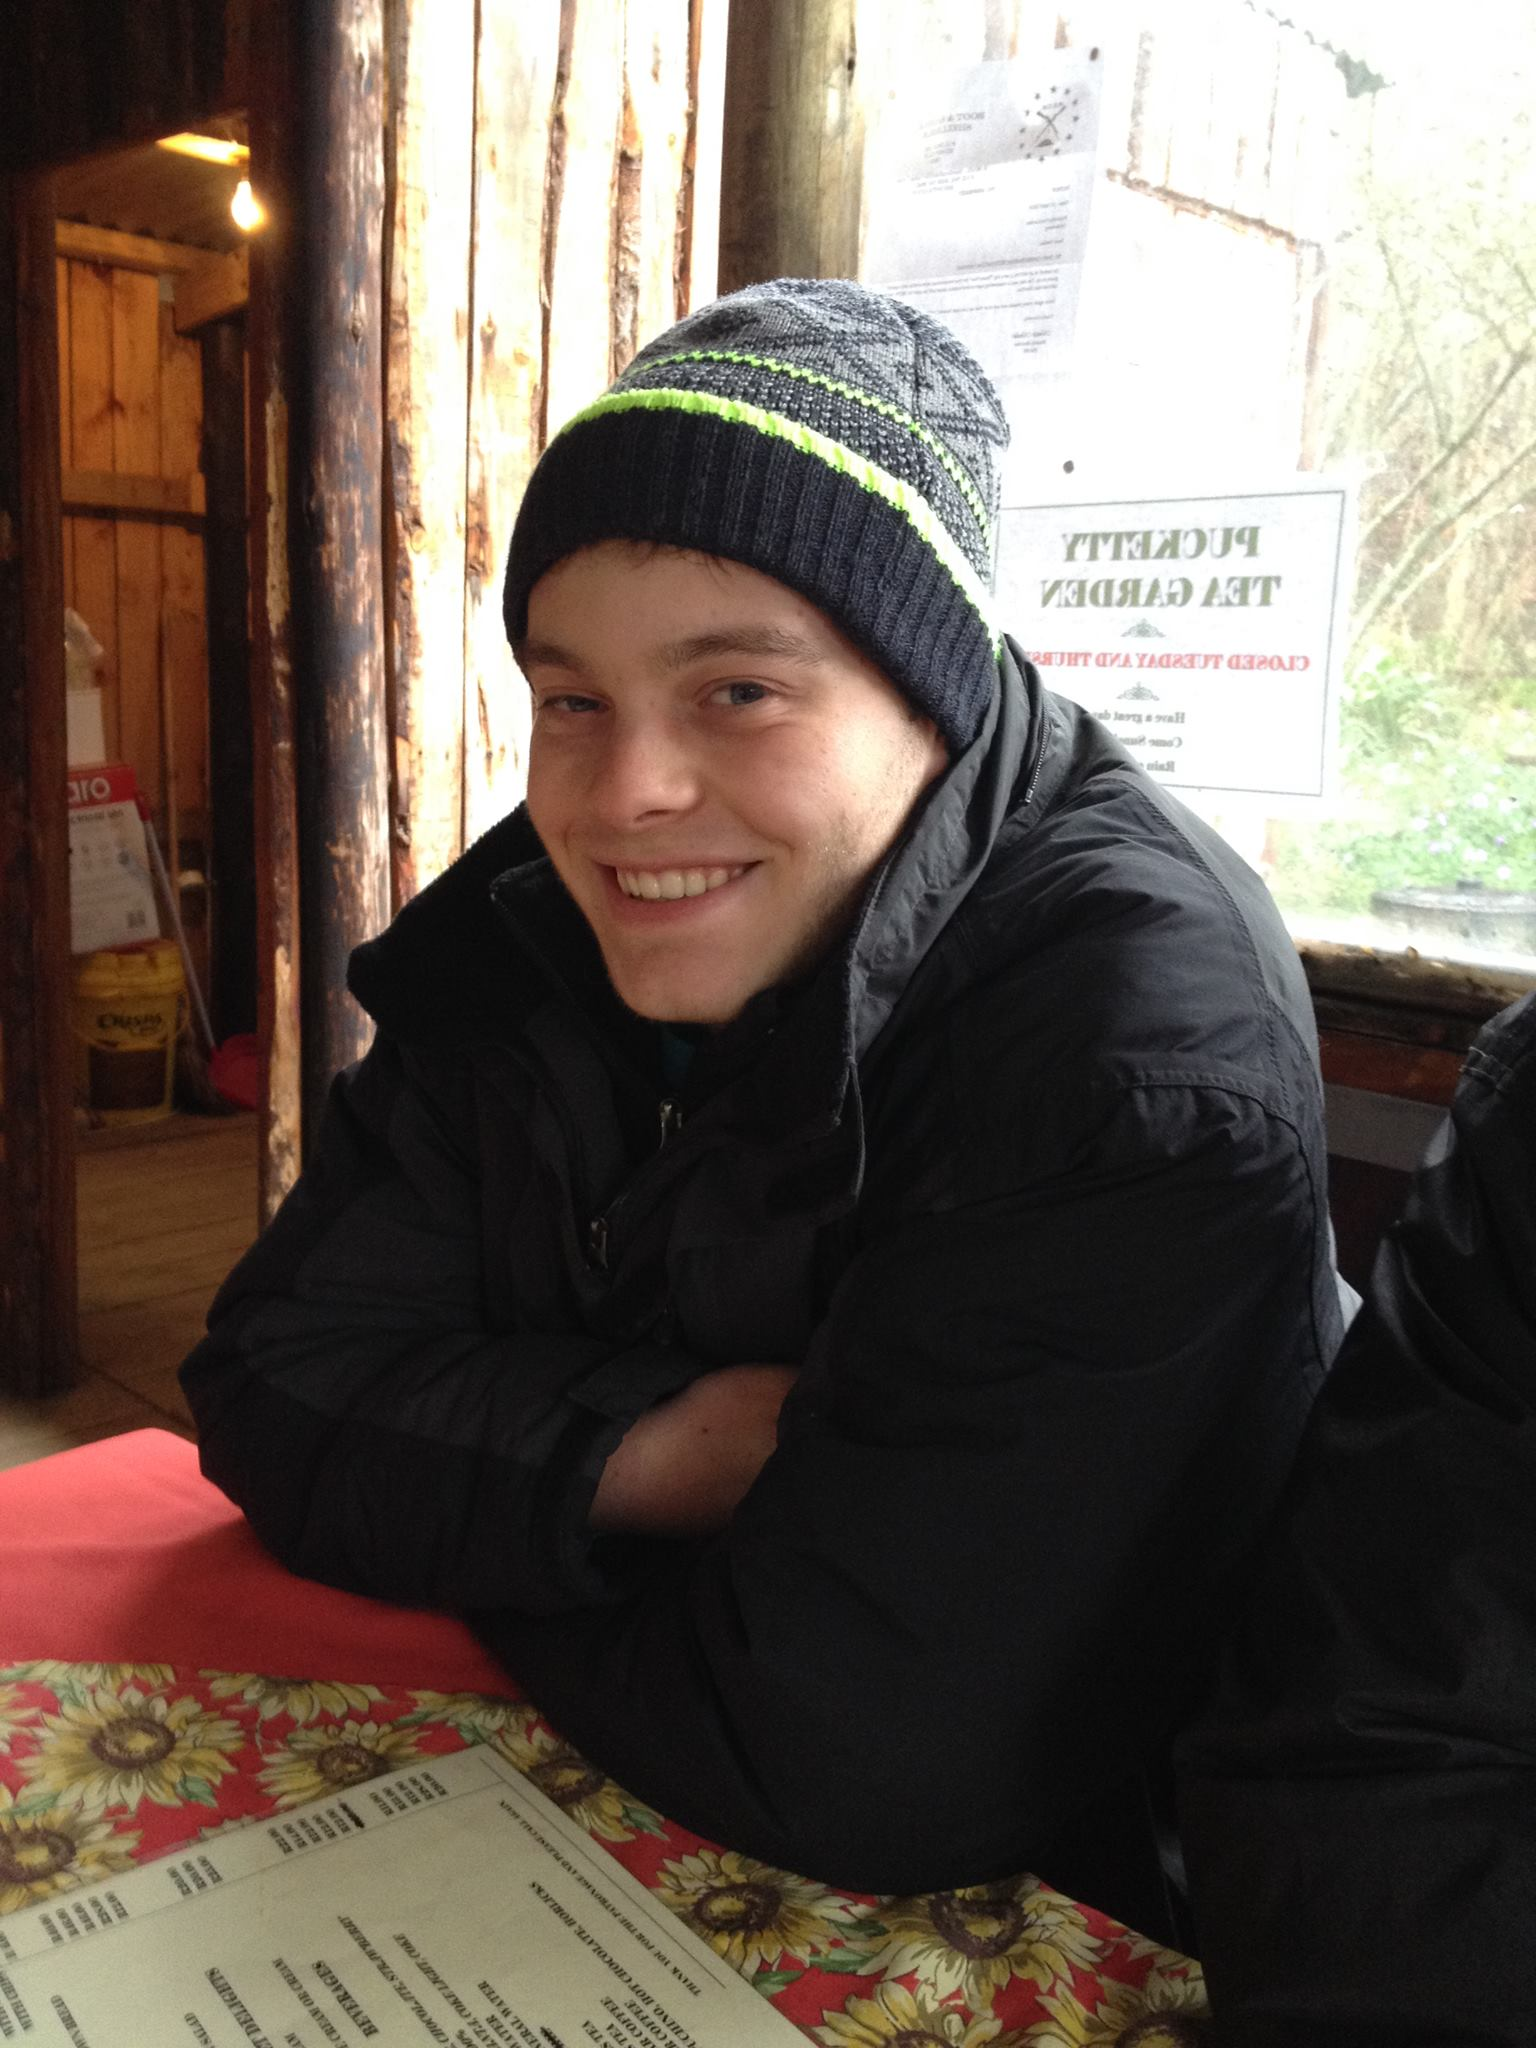
\includegraphics[height=0.3\textheight]{../charl.jpg}
	\end{figure}
	\begin{itemize}
		\item \textbf{Full name:} Lodewyk Charles Meyers
		\item \textbf{My interests:}
			\subitem Gaming
			\subitem Computers
			\subitem Music
			\subitem User experience design
			\subitem Website design
			\subitem Anything new related to technology
		\item \textbf{My technical skills:}
			\subitem Web development skills
			\subitem Database design
			\subitem Java
			\subitem C\#
		\item \textbf{Past experience that might help:}
			\subitem I have collaborated in an Android app made using PhoneGap
		\item \textbf{Non-technical strengths:}
			\subitem I have a high amount of patience
			\subitem Hardworking
			\subitem Eager to learn new things
			\subitem Enjoy trying to solve complex problems
		\item \textbf{What makes me want to do this project?} \newline
		Doing  this project sounds like it can be fun. It sounds like I might learn something new in the Subtropical industry. It will also be interesting to see how the service is being realised to help the farmers determine better yields. Finally it would be nice to learn how to create an app that uses GPS and other technologies needed for this project.
	\end{itemize}
	
	\subsection{EF Bode}
	\begin{figure}[h]
		\centering
		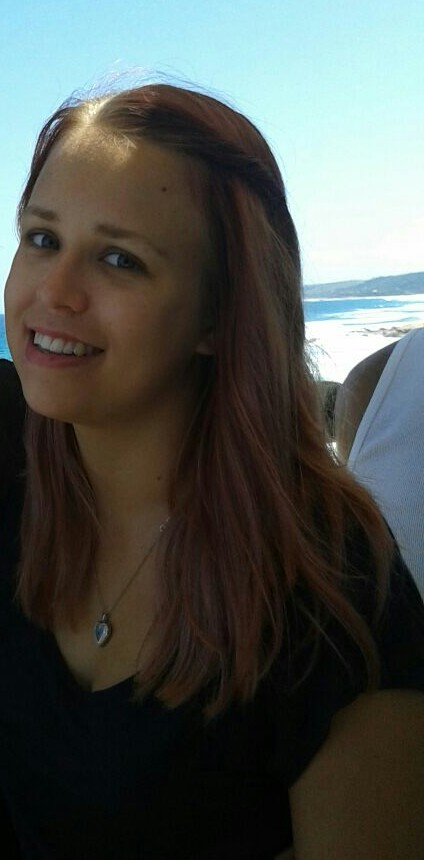
\includegraphics[height=0.3\textheight]{../Liz.jpg}
	\end{figure}
	\begin{itemize}
		\item \textbf{Full Name:} Elizabeth Fae Bode
		\item \textbf{My Interests:}
		\subitem Puzzle Games (eg. Sudoku)
		\subitem Computers
		\subitem Art
		\subitem Music
		\subitem User experience design
		\subitem Website design
		\subitem Gardening
		\subitem Reading books
		
		\item \textbf{My Technical Skills:}
		\subitem Web development skills
		\subitem Database design
		\subitem Java
		\subitem C\#
		\subitem C++
		\subitem Good at writing
		
		\item \textbf{Past Experience that Might Help:} \newline
		I do not have much experience in terms of mobile development but I have always had an eagerness to learn it as it is becoming an increasingly fundamental part of our society. I have slight experience in the agricultural industry as I use to work as a manager at a plant nursery and I learnt a lot about growing plants, the conditions they require and the importance of monitoring the growth of plants in order to increase their success.
		
		\item \textbf{Non-technical Strengths:}
		\subitem Good at decision-making
		\subitem Good at problem-solving
		\subitem Hardworking
		\subitem Organised
		\subitem Responsible
		\subitem Eager to learn new things
		\subitem Perfectionist
		
		\item \textbf{What makes me want to do this project?} \newline
		I have a passion for nature and growing plants in general which I believe will be of assistance in the implementation of this project. This passion also gives me the motivation and the desire to implement this project as I believe it will be an interesting experience that I would love to be involved in 100\% in order to grow my knowledge in every respect.
	\end{itemize}

		\subsection{C Saaiman}
	\begin{figure}[h]
		\centering
		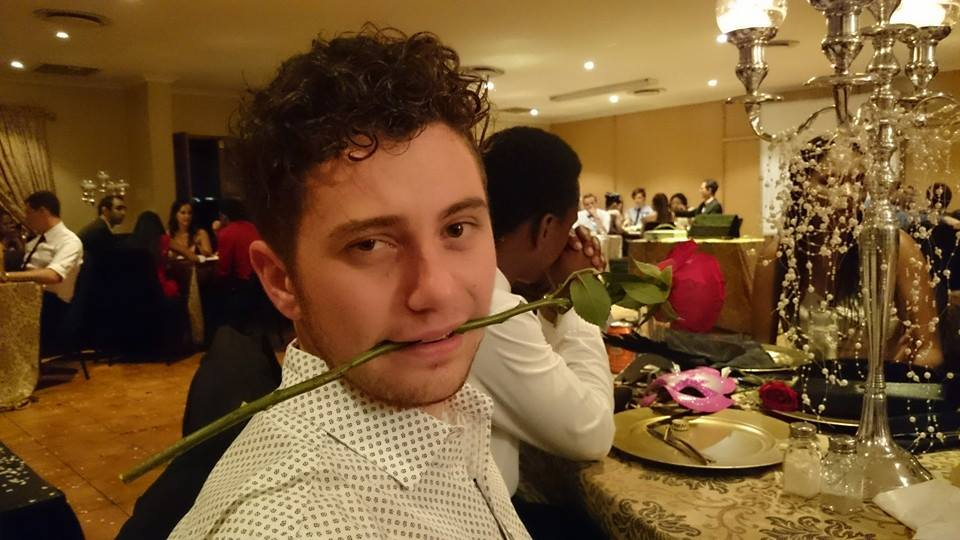
\includegraphics[height=0.3\textheight]{../Saaiman.jpg}
	\end{figure}
    
    \begin{itemize}
    \item \textbf{Full Name:} Christiaan Saaiman
    \item \textbf{My interests:}
    	\subitem Reading books
        \subitem Piano playing
        \subitem Gaming
        \subitem Coding
        \subitem Web Design
        \subitem User Experience Design
        \subitem Cooking and Baking
		\subitem Anime
        \subitem Languages
        	\subsubitem German
            \subsubitem Italian
            \subsubitem Japanese
        \subitem Artificial Intelligence
        \subitem Phones, Computer Hardware and Next-Gen Consoles

	\item \textbf{Technical Skills:}
    	\subitem Web Development Skills
        \subitem Java
        \subitem C++
        
	\item \textbf{Past experience:}
    	\subitem 6 Months intensive Java Training Course
        \subitem 6 Month Internship at Accenture
        	\subsubitem Intense Oracle Systems Training
            \subsubitem Leadership Training and meetings with the MD of Technology
            \subsubitem pitching an idea a colleague and I had.
            \subsubitem Tiger Brands' System upgrade from Oracle Database 11g to 12c
        \subitem Android App development using PhoneGap
    \item \textbf{Non-technical Strengths:}
    	\subitem Excellent Leader, not  afraid of conflict
        \subitem Excellent communicator
        \subitem Curious and eager to take on challenges
        \subitem Problem solver
        \subitem Dedicated and hardworking
        \subitem Creative and spontaneous
        
   \item \textbf{Reason for Project Tender:} \newline
   The project proposal peaked my interest in several ways. Firstly I was curious to extend my knowledge with regards to the subtropical farming that is present in South Africa and how it plays its role as a significant forex earner in our country. Secondly I was delighted to see that there is a need for an application, as I wish to further extend and broaden my knowledge in the field of Mobile Development. This project I believe I will tackle with enthusiasm and grit. Lastly I was also intrigued by the thought of helping farmers with an app to help them better their yield. I want to know more of how this could be further extended to help not only farmers, but other business owners as well.
       
	\end{itemize}
		
	\subsection{M Loosen}
	\begin{figure}[h]
		\centering
		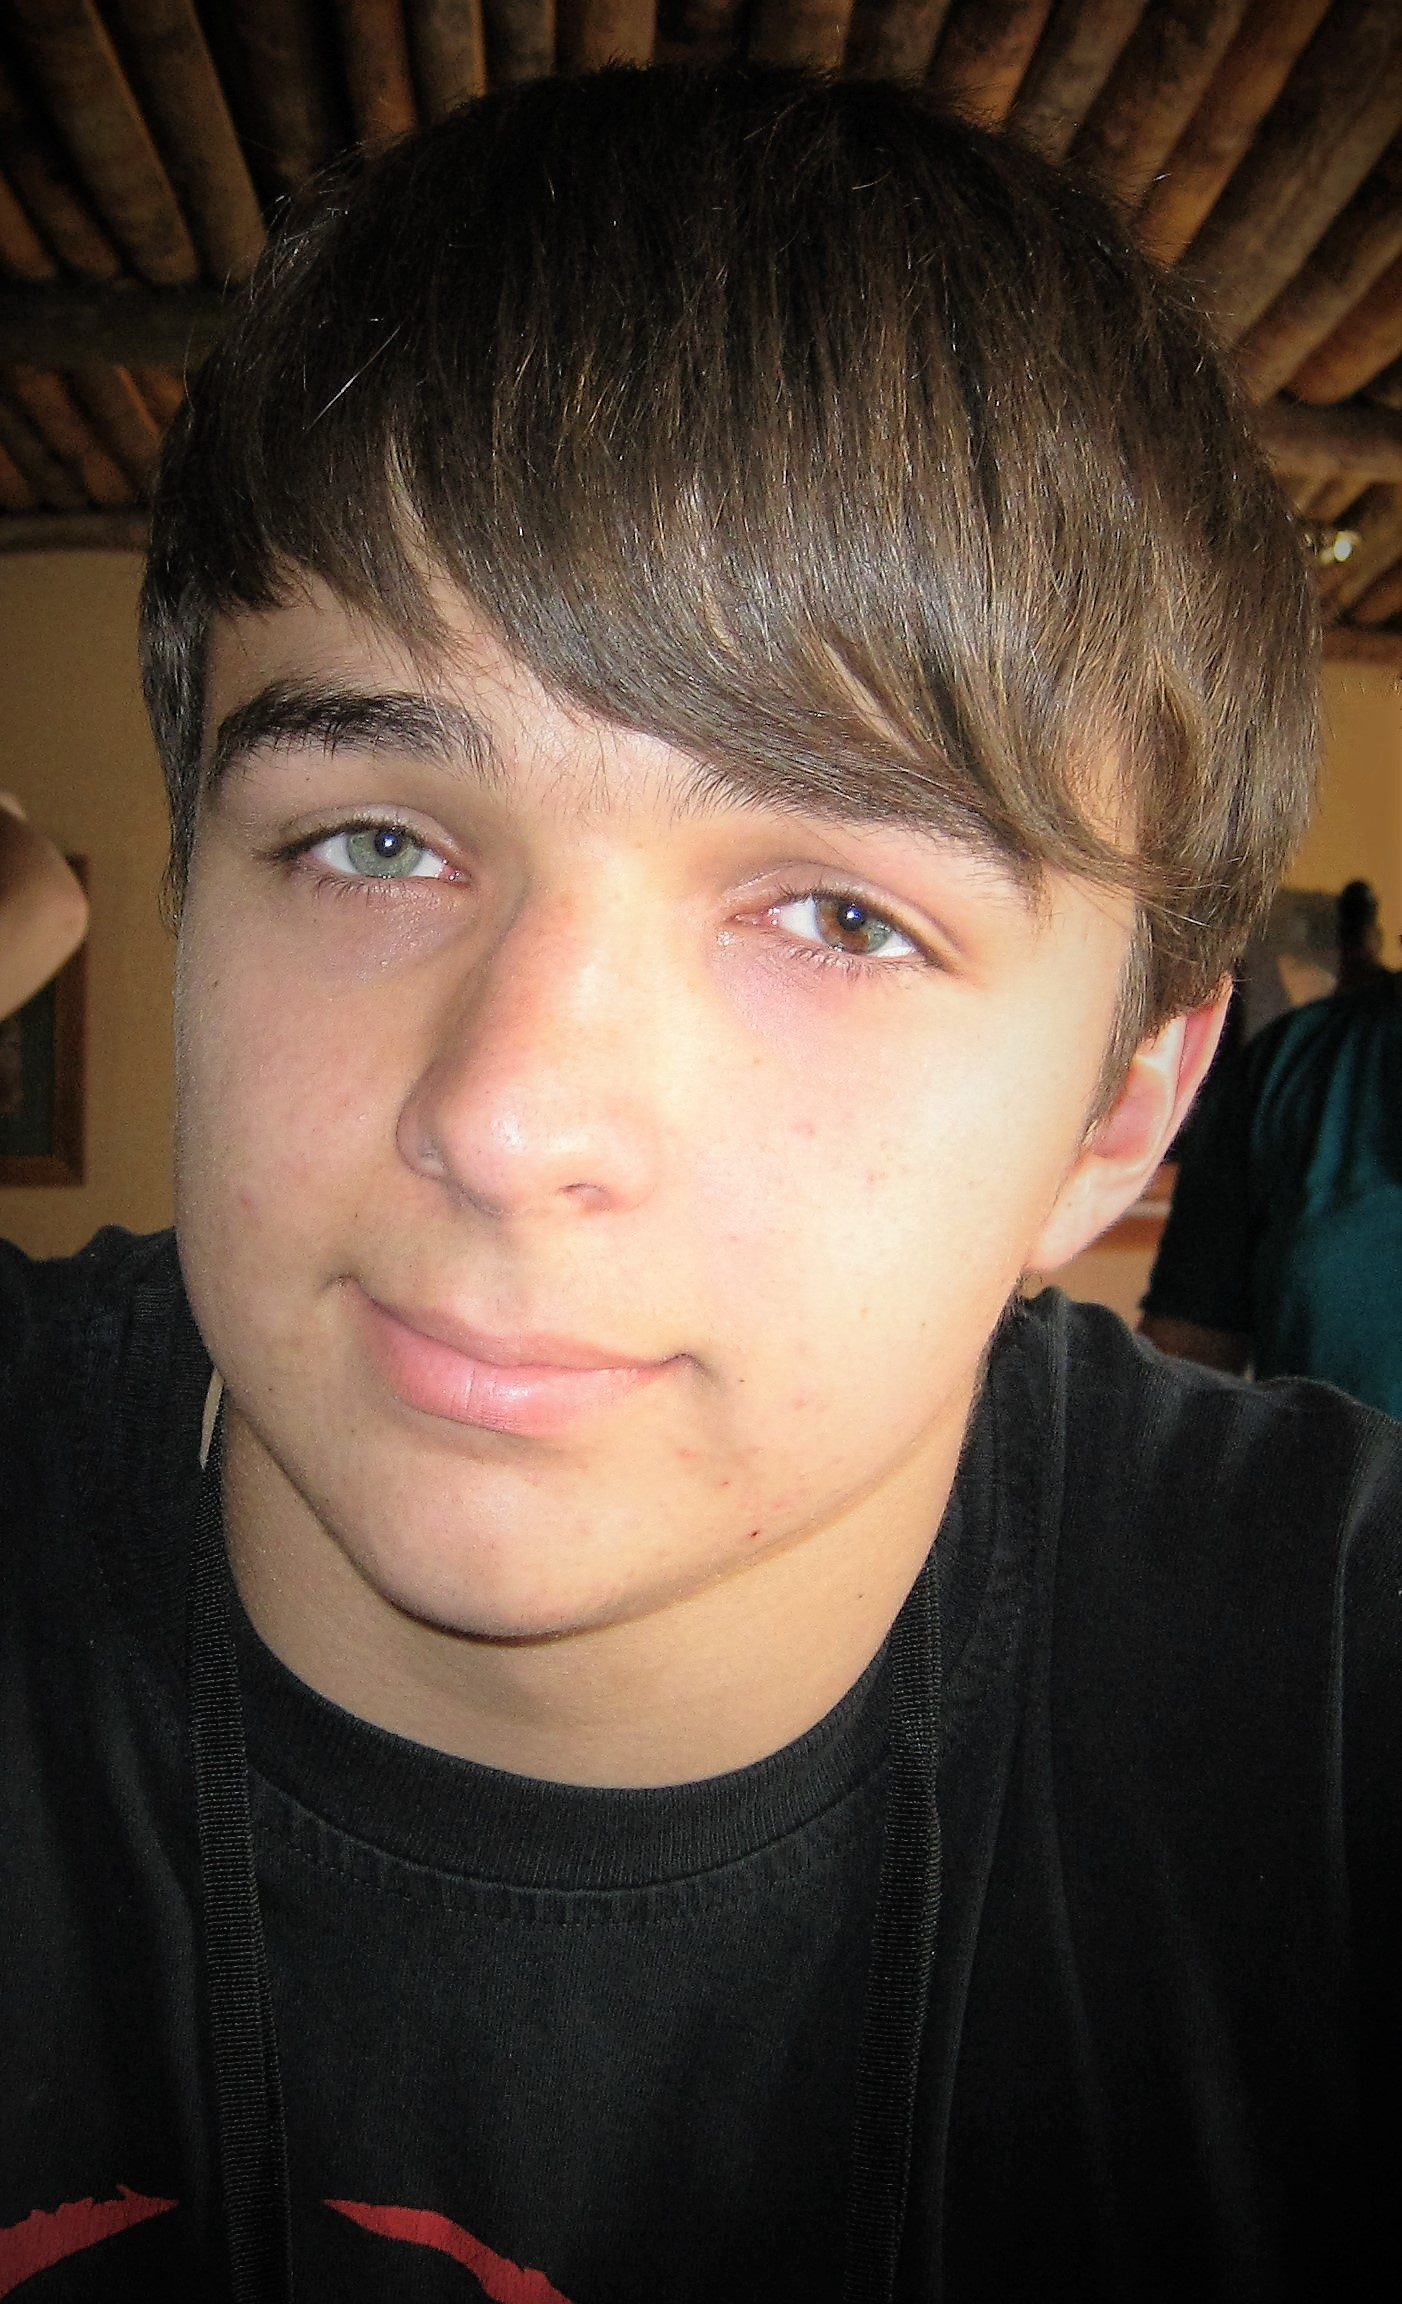
\includegraphics[height=0.3\textheight]{../Michael.jpg}
	\end{figure}
	\begin{itemize}
		\item \textbf{Full Name:} Michael Loosen
		\item \textbf{My Interests:}
		\subitem Gaming
		\subitem Coding
		\subitem Cooking
		\subitem Flying (Pilot)
		\subitem Motorcycles
		\subitem Planes
		\subitem Cars
		\subitem Music
		
		\item \textbf{My Technical Skills:}
		\subitem Database design
		\subitem Java development
		\subitem Web development skills		
		\subitem C\# development
		\subitem C++ development
		\subitem Technical document writing
		
		\item \textbf{Past Experience that Might Help:} \newline
		My father, Dirk Loosen, has been in IT since before I was born and this is what lead to my interest in computers. I have learnt a lot from him, so I might have learnt something from him that could be of use. I also recently had the priveledge of job shadowing him at FNB Bank City. Here I was able to experience a large team of people working on a new application that was being developed using the Agile developement methodology.
		
		\item \textbf{Non-technical Strengths:}
		\subitem Good at problem solving
		\subitem Good at critical analysis
		\subitem Perfectionist		
		\subitem Good at decision making
		\subitem Hardworking
		\subitem Organised
		
		\item \textbf{What makes me want to do this project?} \newline
		I am excited to work on this project because I enjoy creating new applications that can improve our society. To me, technology is a way of benefitting our human race and by doing this project, we will be using technology to improve the execution of an existing process that might put a lot of strain on the process driver, which will be removed or at least eased by this application.
	\end{itemize}
	
	
	\section{Project excecution}
	\begin{itemize}
		\item \textbf{Development Methodology} \newline \newline
		We plan to follow the Agile development methodology as it involves regular communication with the client to ensure the project results in exactly what they want. It also has a focus on the people system and their interactions with it which we believe is way more important than focusing on the processes and tools of the system. We strive to maintain a continues attention to designing the system well and ensuring that all the technical aspects are coherent with the requirements. All of which makes the Agile development methodology perfect for our vision for your project.
		
		\item \textbf{Progress Communication Plan} \newline \newline
		We plan on meeting up with you as the client on a regular basis, either face-to-face or via Skype, whichever is more convenient for you at the time, in order to keep you updated regarding the status of the project and to clarify requirements. We are also willing to communicate either via WhatsApp or email, whichever you prefer, in order to discuss the project and the progress of it, if face-to-face meetings are unable to take place for whatever reasons.

		\item \textbf{Technical Challenges \& Possible Solutions} \newline \newline
		Some of the technical challenges that we might face is our app development for iOS as none of us are experienced in this aspect. We have already made provisions for this by recruiting the help of another developer whos has experience in developing in the iOS environment. They will provide help by guiding us in development, referring us to websites that may improve our understanding and knowledZge and by sharing their knowledge with us. \newline
		Any knowledge that we do not have with regards to the project specific calculations we are determined to study and master. One of us will be appointed to research the problem area and gain as much knowledge as possible. They will then be responsible for a knowledge transfer session in order to share their understanding with the rest fo the team.
		\item \textbf{Technologies we will use for the project:}
			\begin{itemize}
				\item For the front end we will use Cordova along with Ionic as these technologies makes creating hybrid mobile apps easier. This means minimal code will need to be changed to make the app compatible with both Android and iOS. Since this front end is in essence a website and therefore will go nicely with a client/server architecture.
				\item For the backend we will use PHP along with the Laravel framework for PHP. PHP is a very popular web language and is the langauge that most hired web servers run on. Laravel is a new and growing framework for PHP that makes abstracting the database and making RESTful services very easy.
				\item For persistence we will use MySQL. It is a very popular Relational Database Management System that is also iscluded in a lot of hired web servers. Making setup very easy. We also do not anticipate that too much data will be persisted for MySQL to become unreliable.
				\item If no web server is provided we can subscribe to any web hosting service that is very cheap to subscribe to a shared Linux server.
			\end{itemize}
		\item \textbf{What will be delivered to the client on project completion:} \newline \newline
			The aim is to produce a fully functional application that can assist growers with yield data. Our team will strive to produce this application to the best of our abbilities and will ensure that all of the required functionality is implemented correctly and that the application runs smoothly and is user friendly. The client will then receive this application and be able to use it to their benefit.
	\end{itemize}
\end{document}